\chapter{Decidability of Unoriented Trees Realizations Using Logic Engines}
\section{Not All Equal 3 SAT Problem}
\begin{prob}[Not All Equal 3 SAT Problem]\label{prob:Satisfiability-2}%Problem/Question
Give a set of clauses $C$, each containing three boolean variables, can each clause contain at
least one true variable and one false variable?
\end{prob}
\subsection{The Logic Engine}
\begin{figure}[!htbp]
\begin{center}
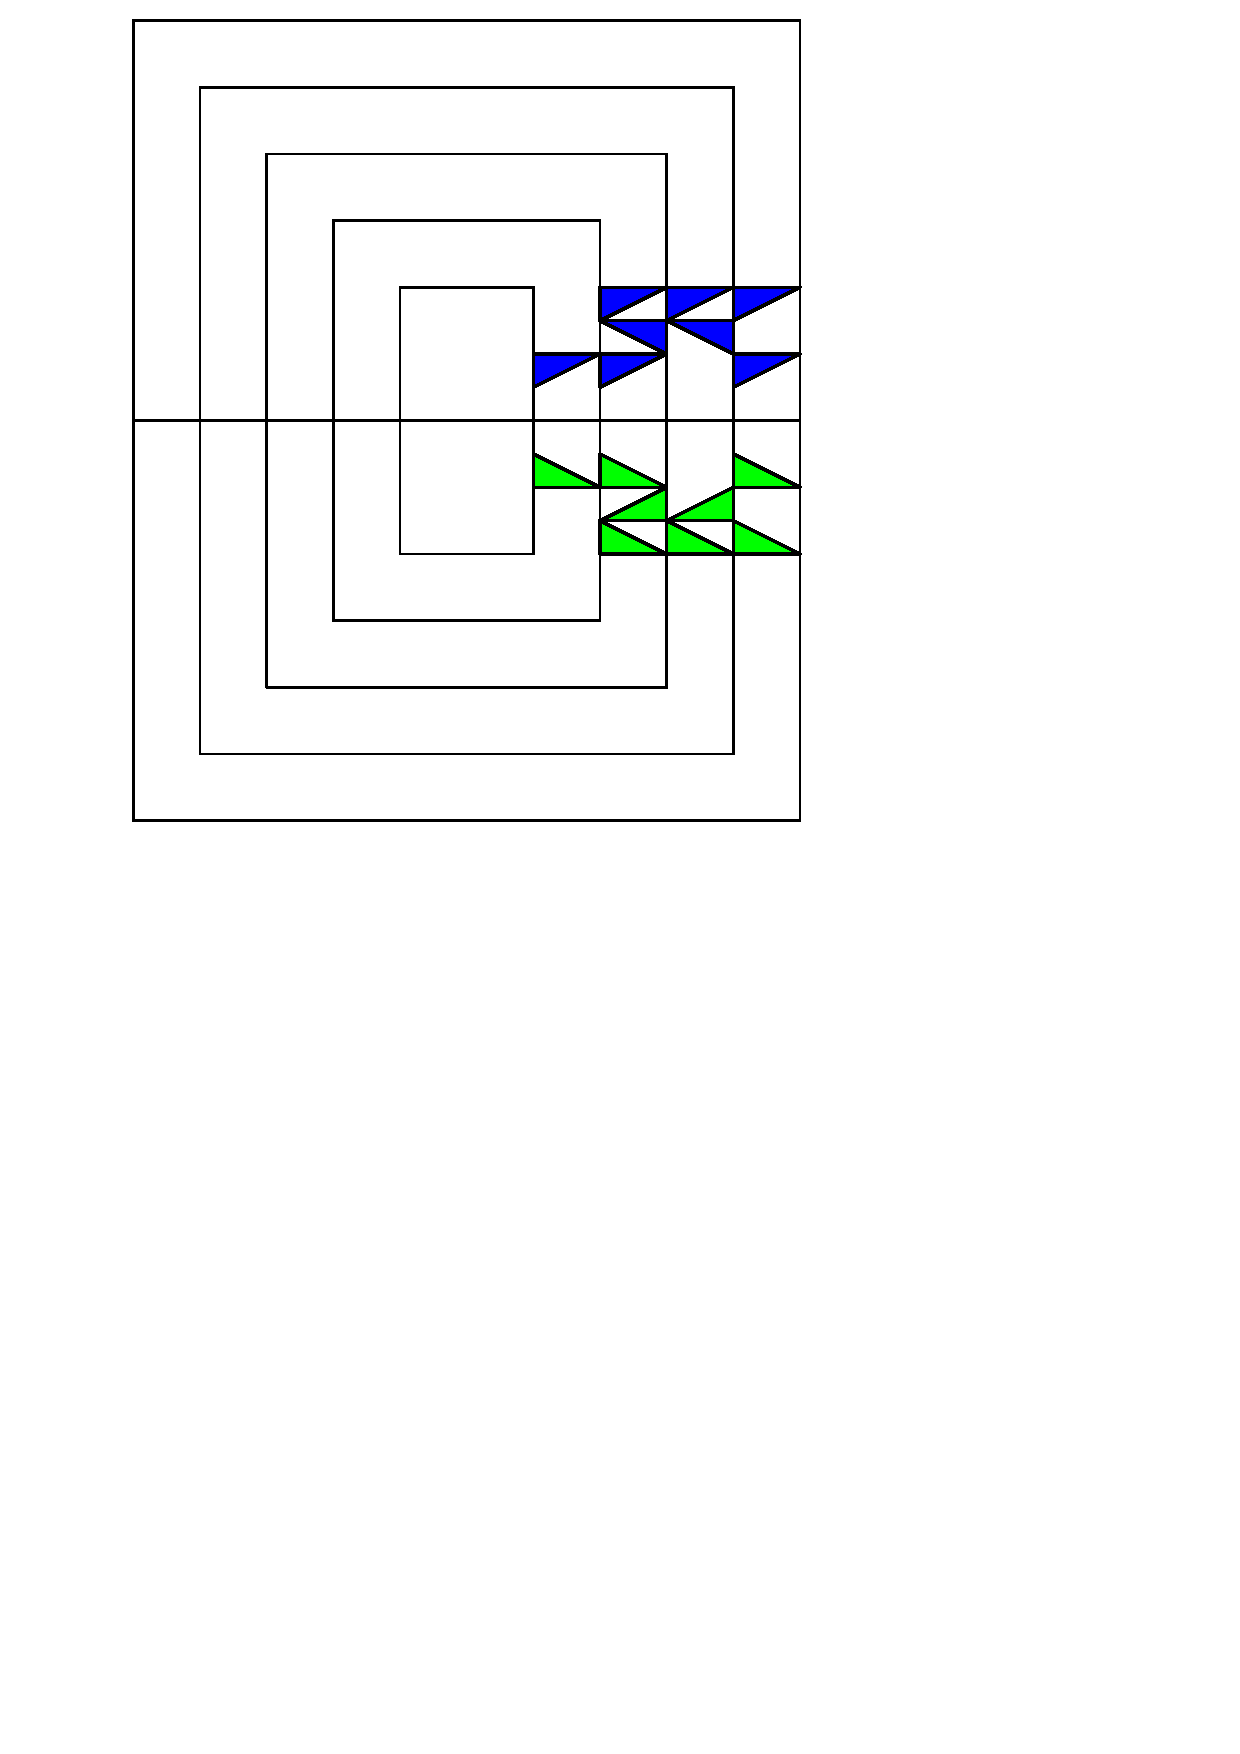
\includegraphics[scale=.66]{graphics/logicengine.pdf}
\caption{A logic engine example.}\label{fig:logicengine-1}
\end{center}
\end{figure}
%add figure of logic engine.
\subsubsection{Construction of the Logic Engine and Encoding of an NAE3SAT Problem on a Logic 
Engine}
% Rigid Frame - A rigid frame that supports the shaft
% Shaft - placed horizontally mid-height of the frame
% Armature - concentric frames contained within the rigid frame supported by the shaft. for each Var
% Chain - for each variable's literal a_j \bar{a}_j,  there exists a chain on that armature
% Flag - flags are for 
The logic engine is a physical model which can encode instances of the NAE3SAT problem.  The 
components of the logic engine are as follows: the rigid frame, the shaft, the armatures,
the chains, and the flags.  Suppose we have an NAE3SAT problem, $P$, with $n$ variables and $m$ 
clauses.  For each variable in $P$, $vj$, there is an \textit{armature}, $A_j$.  The armatures are 
placed concentrically within a \textit{rigid frame}.  A \textit{shaft} placed at mid-height of the 
rigid frame and goes through the armatures.  The armatures can rotate about the shaft.  For each 
clause $C_k$ in $P$, there is are two \textit{links} placed on each armature, $l_{j,k}$ and 
$\bar{l}_{j,k}$. $l_{j,k}$ and $\bar{l}_{j,k}$ place at a height of $k$ and $-k$ respectively on  
each armature.  Every link is flagged except in the case of the following two conditions:
\begin{enumerate}
 \item If the literal $x_j$ is found in clause $C_k$, then $l_{j,k}$ is unflagged.
 \item If the literal $\bar{x}_j$ is found in clause $C_k$, then $\bar{l}_{j,k}$ is unflagged.
\end{enumerate}

% 
% 
%   The \textit{rigid frame} is a rectangular enclosure with a horizontal
% shaft place at mid-height.  The \textit{armatures} are concentric rectangular frames contained
% within the rigid frame.  Each armature can rotate about the shaft; other motions on the armature
% are disallowed.  Given an NAE3SAT, for each variable there is a corresponding armature. On each
% armature, there are chains.  A pair of \textit{chains}, $a_j$ and $\bar{a}_j$ correspond to the
% variable $x_j$ and $\bar{x}_j$ respectively.  The pair is placed on each armature, reflected at a
% height of $h$ above and below the shaft, i.e. one place above the shave at a height of $h$, the
% other placed below the shaft at a height of $-h$.
% %insert an armature graphic
% 
% \subsubsection{Encoding the Logic Engine}
% For each clause of an NAE3SAT, there exists a set of corresponding chains, namely the $h^\text{th}$
% clause is the set of chains on the armatures at the $h^\text{th}$ row above and below the shaft. A
% chain is \textit{flagged} if the corresponding variable resides within the clause.  The flag can
% point in either the left or right directions indicating a truth assignment for that variable within
% the clause.  A flag is attached to the $i^\text{th}$ chain of every $a_j^\text{th}$ and
% $\bar{a}_j^\text{th}$ chain with the following exceptions:
% \begin{enumerate}
%  \item if the variable $x_j$  is in clause $C_i$, then link $i$ of $a_j$ is unflagged,
%  \item if the variable $\bar{x}_j$ is in clause $C_i$, then link $i$ of $a_j$ is unflagged.
% \end{enumerate}
\begin{thm}\label{thm:Satisfiability-1}
 An instance of $NAE3SAT$ is a ``yes'' instance if and only if the corresponding logic engine has a
flat, collision-free configuration.
\end{thm}
\begin{pf}
%  If an instance of $NAE3SAT$ is a ``yes'', then every clause in $C$ contains at least one true
% variable and one false variable.  Now suppose the following truth assignment:

\end{pf}
